% Created by tikzDevice version 0.10.1 on 2016-08-26 10:26:47
% !TEX encoding = UTF-8 Unicode
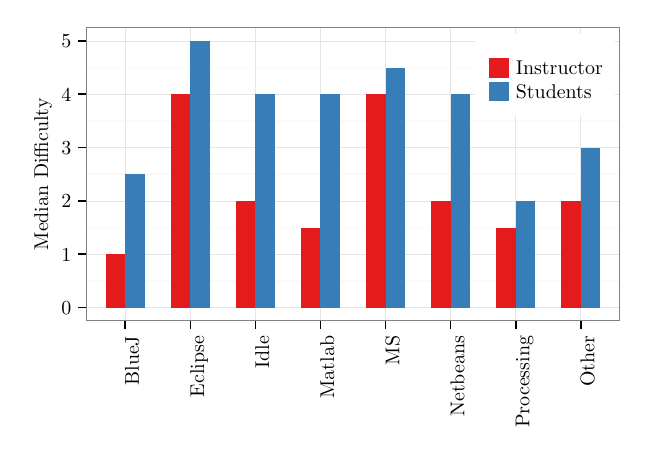
\begin{tikzpicture}[x=1pt,y=1pt]
\definecolor{fillColor}{RGB}{255,255,255}
\path[use as bounding box,fill=fillColor,fill opacity=0.00] (0,0) rectangle (216.81,144.54);
\begin{scope}
\path[clip] (  0.00,  0.00) rectangle (216.81,144.54);
\definecolor{drawColor}{RGB}{255,255,255}
\definecolor{fillColor}{RGB}{255,255,255}

\path[draw=drawColor,line width= 0.6pt,line join=round,line cap=round,fill=fillColor] ( -0.00,  0.00) rectangle (216.81,144.54);
\end{scope}
\begin{scope}
\path[clip] ( 21.16, 38.59) rectangle (213.96,144.54);
\definecolor{fillColor}{RGB}{255,255,255}

\path[fill=fillColor] ( 21.16, 38.59) rectangle (213.96,144.54);
\definecolor{drawColor}{gray}{0.98}

\path[draw=drawColor,line width= 0.6pt,line join=round] ( 21.16, 53.04) --
	(213.96, 53.04);

\path[draw=drawColor,line width= 0.6pt,line join=round] ( 21.16, 72.30) --
	(213.96, 72.30);

\path[draw=drawColor,line width= 0.6pt,line join=round] ( 21.16, 91.57) --
	(213.96, 91.57);

\path[draw=drawColor,line width= 0.6pt,line join=round] ( 21.16,110.83) --
	(213.96,110.83);

\path[draw=drawColor,line width= 0.6pt,line join=round] ( 21.16,130.09) --
	(213.96,130.09);
\definecolor{drawColor}{gray}{0.90}

\path[draw=drawColor,line width= 0.2pt,line join=round] ( 21.16, 43.41) --
	(213.96, 43.41);

\path[draw=drawColor,line width= 0.2pt,line join=round] ( 21.16, 62.67) --
	(213.96, 62.67);

\path[draw=drawColor,line width= 0.2pt,line join=round] ( 21.16, 81.93) --
	(213.96, 81.93);

\path[draw=drawColor,line width= 0.2pt,line join=round] ( 21.16,101.20) --
	(213.96,101.20);

\path[draw=drawColor,line width= 0.2pt,line join=round] ( 21.16,120.46) --
	(213.96,120.46);

\path[draw=drawColor,line width= 0.2pt,line join=round] ( 21.16,139.72) --
	(213.96,139.72);

\path[draw=drawColor,line width= 0.2pt,line join=round] ( 35.27, 38.59) --
	( 35.27,144.54);

\path[draw=drawColor,line width= 0.2pt,line join=round] ( 58.78, 38.59) --
	( 58.78,144.54);

\path[draw=drawColor,line width= 0.2pt,line join=round] ( 82.29, 38.59) --
	( 82.29,144.54);

\path[draw=drawColor,line width= 0.2pt,line join=round] (105.80, 38.59) --
	(105.80,144.54);

\path[draw=drawColor,line width= 0.2pt,line join=round] (129.32, 38.59) --
	(129.32,144.54);

\path[draw=drawColor,line width= 0.2pt,line join=round] (152.83, 38.59) --
	(152.83,144.54);

\path[draw=drawColor,line width= 0.2pt,line join=round] (176.34, 38.59) --
	(176.34,144.54);

\path[draw=drawColor,line width= 0.2pt,line join=round] (199.86, 38.59) --
	(199.86,144.54);
\definecolor{fillColor}{RGB}{55,126,184}

\path[fill=fillColor] ( 35.27, 43.41) rectangle ( 42.32, 91.57);
\definecolor{fillColor}{RGB}{228,26,28}

\path[fill=fillColor] ( 28.21, 43.41) rectangle ( 35.27, 62.67);
\definecolor{fillColor}{RGB}{55,126,184}

\path[fill=fillColor] ( 58.78, 43.41) rectangle ( 65.83,139.72);
\definecolor{fillColor}{RGB}{228,26,28}

\path[fill=fillColor] ( 51.72, 43.41) rectangle ( 58.78,120.46);
\definecolor{fillColor}{RGB}{55,126,184}

\path[fill=fillColor] ( 82.29, 43.41) rectangle ( 89.35,120.46);
\definecolor{fillColor}{RGB}{228,26,28}

\path[fill=fillColor] ( 75.24, 43.41) rectangle ( 82.29, 81.93);
\definecolor{fillColor}{RGB}{55,126,184}

\path[fill=fillColor] (105.80, 43.41) rectangle (112.86,120.46);
\definecolor{fillColor}{RGB}{228,26,28}

\path[fill=fillColor] ( 98.75, 43.41) rectangle (105.80, 72.30);
\definecolor{fillColor}{RGB}{55,126,184}

\path[fill=fillColor] (129.32, 43.41) rectangle (136.37,130.09);
\definecolor{fillColor}{RGB}{228,26,28}

\path[fill=fillColor] (122.26, 43.41) rectangle (129.32,120.46);
\definecolor{fillColor}{RGB}{55,126,184}

\path[fill=fillColor] (152.83, 43.41) rectangle (159.88,120.46);
\definecolor{fillColor}{RGB}{228,26,28}

\path[fill=fillColor] (145.78, 43.41) rectangle (152.83, 81.93);
\definecolor{fillColor}{RGB}{55,126,184}

\path[fill=fillColor] (176.34, 43.41) rectangle (183.40, 81.93);
\definecolor{fillColor}{RGB}{228,26,28}

\path[fill=fillColor] (169.29, 43.41) rectangle (176.34, 72.30);
\definecolor{fillColor}{RGB}{55,126,184}

\path[fill=fillColor] (199.86, 43.41) rectangle (206.91,101.20);
\definecolor{fillColor}{RGB}{228,26,28}

\path[fill=fillColor] (192.80, 43.41) rectangle (199.86, 81.93);
\definecolor{drawColor}{gray}{0.50}

\path[draw=drawColor,line width= 0.6pt,line join=round,line cap=round] ( 21.16, 38.59) rectangle (213.96,144.54);
\end{scope}
\begin{scope}
\path[clip] (  0.00,  0.00) rectangle (216.81,144.54);
\definecolor{drawColor}{RGB}{0,0,0}

\node[text=drawColor,anchor=base east,inner sep=0pt, outer sep=0pt, scale=  0.72] at ( 15.76, 40.93) {0};

\node[text=drawColor,anchor=base east,inner sep=0pt, outer sep=0pt, scale=  0.72] at ( 15.76, 60.19) {1};

\node[text=drawColor,anchor=base east,inner sep=0pt, outer sep=0pt, scale=  0.72] at ( 15.76, 79.45) {2};

\node[text=drawColor,anchor=base east,inner sep=0pt, outer sep=0pt, scale=  0.72] at ( 15.76, 98.72) {3};

\node[text=drawColor,anchor=base east,inner sep=0pt, outer sep=0pt, scale=  0.72] at ( 15.76,117.98) {4};

\node[text=drawColor,anchor=base east,inner sep=0pt, outer sep=0pt, scale=  0.72] at ( 15.76,137.24) {5};
\end{scope}
\begin{scope}
\path[clip] (  0.00,  0.00) rectangle (216.81,144.54);
\definecolor{drawColor}{RGB}{0,0,0}

\path[draw=drawColor,line width= 0.6pt,line join=round] ( 18.16, 43.41) --
	( 21.16, 43.41);

\path[draw=drawColor,line width= 0.6pt,line join=round] ( 18.16, 62.67) --
	( 21.16, 62.67);

\path[draw=drawColor,line width= 0.6pt,line join=round] ( 18.16, 81.93) --
	( 21.16, 81.93);

\path[draw=drawColor,line width= 0.6pt,line join=round] ( 18.16,101.20) --
	( 21.16,101.20);

\path[draw=drawColor,line width= 0.6pt,line join=round] ( 18.16,120.46) --
	( 21.16,120.46);

\path[draw=drawColor,line width= 0.6pt,line join=round] ( 18.16,139.72) --
	( 21.16,139.72);
\end{scope}
\begin{scope}
\path[clip] (  0.00,  0.00) rectangle (216.81,144.54);
\definecolor{drawColor}{RGB}{0,0,0}

\path[draw=drawColor,line width= 0.6pt,line join=round] ( 35.27, 35.59) --
	( 35.27, 38.59);

\path[draw=drawColor,line width= 0.6pt,line join=round] ( 58.78, 35.59) --
	( 58.78, 38.59);

\path[draw=drawColor,line width= 0.6pt,line join=round] ( 82.29, 35.59) --
	( 82.29, 38.59);

\path[draw=drawColor,line width= 0.6pt,line join=round] (105.80, 35.59) --
	(105.80, 38.59);

\path[draw=drawColor,line width= 0.6pt,line join=round] (129.32, 35.59) --
	(129.32, 38.59);

\path[draw=drawColor,line width= 0.6pt,line join=round] (152.83, 35.59) --
	(152.83, 38.59);

\path[draw=drawColor,line width= 0.6pt,line join=round] (176.34, 35.59) --
	(176.34, 38.59);

\path[draw=drawColor,line width= 0.6pt,line join=round] (199.86, 35.59) --
	(199.86, 38.59);
\end{scope}
\begin{scope}
\path[clip] (  0.00,  0.00) rectangle (216.81,144.54);
\definecolor{drawColor}{RGB}{0,0,0}

\node[text=drawColor,rotate= 90.00,anchor=base east,inner sep=0pt, outer sep=0pt, scale=  0.72] at ( 40.22, 33.19) {BlueJ};

\node[text=drawColor,rotate= 90.00,anchor=base east,inner sep=0pt, outer sep=0pt, scale=  0.72] at ( 63.74, 33.19) {Eclipse};

\node[text=drawColor,rotate= 90.00,anchor=base east,inner sep=0pt, outer sep=0pt, scale=  0.72] at ( 87.25, 33.19) {Idle};

\node[text=drawColor,rotate= 90.00,anchor=base east,inner sep=0pt, outer sep=0pt, scale=  0.72] at (110.76, 33.19) {Matlab};

\node[text=drawColor,rotate= 90.00,anchor=base east,inner sep=0pt, outer sep=0pt, scale=  0.72] at (134.28, 33.19) {MS};

\node[text=drawColor,rotate= 90.00,anchor=base east,inner sep=0pt, outer sep=0pt, scale=  0.72] at (157.79, 33.19) {Netbeans};

\node[text=drawColor,rotate= 90.00,anchor=base east,inner sep=0pt, outer sep=0pt, scale=  0.72] at (181.30, 33.19) {Processing};

\node[text=drawColor,rotate= 90.00,anchor=base east,inner sep=0pt, outer sep=0pt, scale=  0.72] at (204.82, 33.19) {Other};
\end{scope}
\begin{scope}
\path[clip] (  0.00,  0.00) rectangle (216.81,144.54);
\definecolor{drawColor}{RGB}{0,0,0}

\node[text=drawColor,rotate= 90.00,anchor=base,inner sep=0pt, outer sep=0pt, scale=  0.72] at (  7.36, 91.57) {Median Difficulty};
\end{scope}
\begin{scope}
\path[clip] (  0.00,  0.00) rectangle (216.81,144.54);
\definecolor{fillColor}{RGB}{255,255,255}

\path[fill=fillColor] (161.80,112.98) rectangle (212.15,142.20);
\end{scope}
\begin{scope}
\path[clip] (  0.00,  0.00) rectangle (216.81,144.54);
\definecolor{fillColor}{RGB}{228,26,28}

\path[fill=fillColor] (166.78,126.49) rectangle (173.89,133.61);
\end{scope}
\begin{scope}
\path[clip] (  0.00,  0.00) rectangle (216.81,144.54);
\definecolor{fillColor}{RGB}{55,126,184}

\path[fill=fillColor] (166.78,117.96) rectangle (173.89,125.07);
\end{scope}
\begin{scope}
\path[clip] (  0.00,  0.00) rectangle (216.81,144.54);
\definecolor{drawColor}{RGB}{0,0,0}

\node[text=drawColor,anchor=base west,inner sep=0pt, outer sep=0pt, scale=  0.72] at (176.41,127.57) {Instructor};
\end{scope}
\begin{scope}
\path[clip] (  0.00,  0.00) rectangle (216.81,144.54);
\definecolor{drawColor}{RGB}{0,0,0}

\node[text=drawColor,anchor=base west,inner sep=0pt, outer sep=0pt, scale=  0.72] at (176.41,119.03) {Students};
\end{scope}
\end{tikzpicture}
